\chapter{应对项目风险}
\section{项目风险与项目风险管理}
\subsection{风险与项目风险}
风险是指对无法达到预定目标的可能性和结果的一种测评,是可能给项目的成功带来威胁或损害的可能性。
\par 风险包含两个要素:一是某事件发生的可能性;二是该事件发生所带来的影响。
\par 风险的特征:风险的客观性、风险的不确定性、风险事件的随机性、风险的相对性、风险的可变性、风险的阶段性。
\par 项目风险是指由于项目所处环境和条件的不确定性,项目的最终结果与项目利害关系人的期望产生背离,并给项目干系人带来损失的可能性。
\par 项目风险产生的原因主要是由项目的不确定性所造成的;而不确定性是由项目团队无法充分认识项目未来的发展和变化所造成的;
\par 注:
\begin{itemize}
	\item 项目风险贯穿整个项目生命周期,并且项目的不同阶段会有不同的风险。
	\item 风险随着项目的进展而变化,其不确定性一般会逐渐减少。
\end{itemize}
\par 其他关键词:风险的分类。
\subsection{IT项目风险成本}
风险事故造成的损失或减少的收益以及为防止发生风险事故采取的预防措施而支付的费用,都构成了风险成本。
\par 风险成本包括:有形成本、无形成本以及预防与控制风险的费用。  
\subsection{项目风险管理}
项目风险管理:项目管理班子通过风险识别、估计、评价,并以此为基础合理地使用多种管理方法、技术和手段对项目活动涉及的风险实行有效的控制,采取主动行动,创造条件,尽量扩大风险事件的有利结果,妥善处理风险事故造成的不利后果,以最少的成本保证安全、可靠地实现项目的总目标。 
\par 项目风险管理的特点:
\begin{enumerate}
	\item 项目风险管理是为减轻潜在的不利事件对项目的影响而采取的一项活动。
	\item 风险管理是一种投资,需要成本。
	\item 在任何情况下,项目风险管理的成本不应超过项目潜在的收益。
	\item 需要努力在项目的各个方面寻找风险和机会之间的平衡。
\end{enumerate}
\subsection{IT项目风险管理过程}
\begin{figure}[!h]
	\centering
	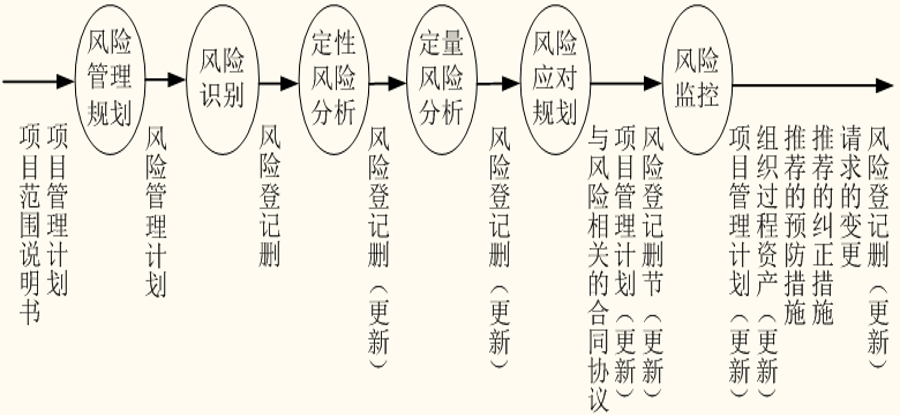
\includegraphics[width=0.8\textwidth]{image/10-1}
	\caption{IT项目风险管理过程}
\end{figure}
\begin{itemize}
	\item 风险管理规划:决定如何开展项目风险管理活动。
	\item 风险识别:判断风险对项目的影响,以书面形式记录特点。
	\item 定性风险分析:对风险进行排序,以便随后进一步分析。
	\item 定量风险分析:对识别的风险进行量化分析。
	\item 风险应对规划:根据项目目标制定风险应对方案。
	\item 风险监控:在整个项目生命周期中,跟踪已识别的风险、监测残余风险、识别新风险和实施风险应对计划,并对其有效性进行评估。
\end{itemize}
\section{风险管理规划}
\subsection{风险管理规划的概念}
风险管理规划是规划和设计如何进行风险管理的过程,记录了管理整个项目过程中所出现风险的程序。
\par 风险管理规划包括定义项目组织及成员风险管理的行动方案及方式,选择合适的风险管理方法,为风险管理活动提供充足的资源和时间,并确立风险评估的基础。 
\par 项目风险管理规划的成果:项目风险管理计划书。
\par 风险管理规划和实施阶段的基本任务:把风险事故的后果尽量限制在可接受的水平上。
\par \textbf{风险应急计划}是指一项已识别的风险事件发生时,项目团队将采取的预先确定的措施。
\par 风险应对的主要选择包括风险预防、风险规避、风险转移、风险减轻、风险自留以及损失控制等。
\subsection{IT项目风险管理计划}
风险管理规划的主要成果是风险管理计划,它描述如何安排与实施项目风险管理,主要包括:
\begin{itemize}
	\item 风险管理方法论
	\item 风险管理相关活动的岗位职责说明
	\item 风险管理活动的预算和进度
	\item 用于定性和定量分析的记分描述和说明方法
	\item 风险的阀限值
	\item 风险管理活动的报告格式
	\item 有关项目团队如何跟踪和记录这些风险活动的描述
\end{itemize}
\section{风险识别}
风险识别就是采用系统化的方法,识别出项目中已知的和可预测到的风险。
\subsection{IT项目风险识别的过程}
 风险识别包括确定风险的来源、风险产生的条件,描述风险特征和确定哪些风险事件有可能影响整个项目。
\par  风险识别应当在IT项目的生命周期自始至终定期进行。风险识别可分为三步进行:
\begin{itemize}
	\item 收集资料
	\item 估计项目风险形势
	\item 根据直接或间接的症状将潜在的风险识别出来
\end{itemize}
\subsection{风险识别的方法}
\begin{itemize}
	\item 文件审查: 对项目计划、假设、先前的项目文档和其他信息等项目文件进行系统和结构性的审查。
	\item 信息收集技术: 包括德尔菲法、头脑风暴法、访谈法、SWOT分析法。
	\item 检查表:用来记录和整理数据的常用工具。
	\item 假设分析:根据一套假定、设想或假设进行构思与制定。
	\item 图解技术:主要包括因果图、系统或过程流程图等。
\end{itemize}
\begin{figure}[!h]
	\centering
	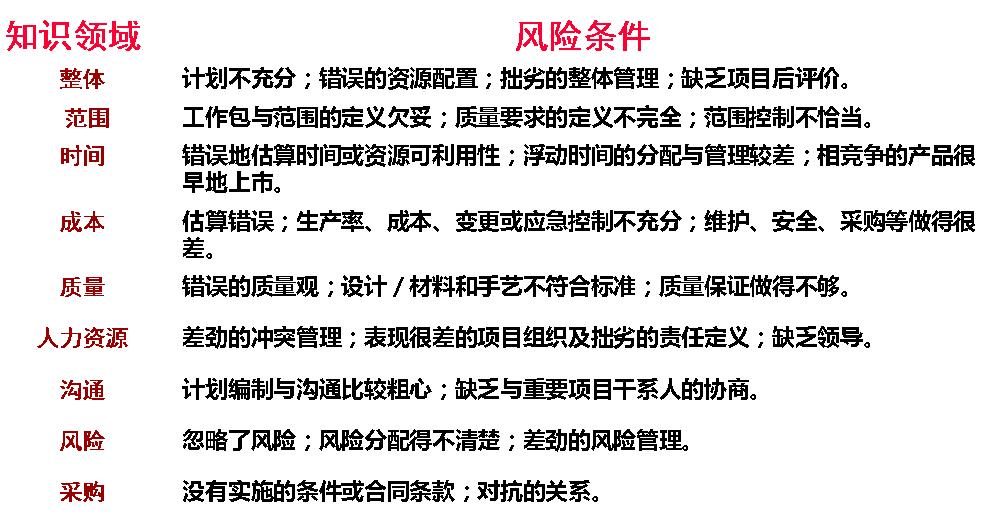
\includegraphics[width=\textwidth]{image/10-2}
	\caption{与各知识领域相关的可能风险条件}
\end{figure}
\subsection{风险登记册}
风险识别之后应把识别的成果整理出来,整理的结果载入到风险登记册中。
\par 风险识别过程将形成项目管理计划中风险登记册的最初记录。
\par 主要依据:已识别风险清单、潜在应对措施清单、风险根本原因、风险类别更新。
\section{定性风险分析}
定性风险分析是指对已识别风险的影响和可能性大小的评估过程。该过程按风险对项目目标潜在影响的轻重缓急进行排序,并为定量风险分析奠定基础。
\par 定性风险分析过程需要使用风险管理规划过程和风险识别过程的成果。
\par 定性风险分析过程完成后,可进入定量风险分析过程或直接进入风险应对规划过程。
\subsection{IT项目定性风险分析的目的}
通过项目风险进行定性分析,可以达到目的:
\begin{enumerate}
	\item 确认项目风险的来源
	\item 确认项目风险的性质
	\item 估计项目风险的影响程度
	\item 为项目风险的定量分析提供条件
\end{enumerate}
\subsection{定性风险分析的方法}
定性风险分析的方法:风险概率与影响评估、
概率和影响矩阵、十大风险事项跟踪、
风险数据质量分析、风险分类、风险紧迫性评估。
\subsection{更新风险登记册}
定性风险分析成果主要是更新的风险登记册。
对风险登记册进行更新的内容包括:
\begin{itemize}
	\item 按照轻重缓急排序的项目风险清单
	\item 按照类别分类的风险 
	\item 需要在近期采取应对措施的风险清单 
	\item 需要进一步分析与应对的风险清单 
	\item 低优先级风险观察清单 
	\item 定性风险分析结果的趋势 
\end{itemize}
\section{定量风险分析}
定量风险分析的目标是量化分析每一个风险的概率及其对项目目标造成的后果,分析项目总体风险的程度。
\subsection{定量风险分析概述}
定量风险分析是指对定性风险分析过程中作为项目需求存在的重大影响而排序在先的风险进行分析,并就风险分配一个数值。
\par 定量风险分析是在不确定情况下进行决策的一种量化方法,该过程通过采用决策树分析和模拟技术等得到如下结果。
\begin{itemize}
	\item 对项目目标以及实现项目目标的概率进行评估并量化。
	\item 通过量化各项风险对项目总体风险的影响,确定需要特别重视的风险。
	\item 在考虑项目风险的情况下,确定可以实现的切合实际的成本、进度或范围目标。
	\item 在某些条件或结果不确定时,确定最佳的项目管理决策。
\end{itemize}
\subsection{软件项目定量风险分析的方法}
\begin{itemize}
	\item 数据收集和表示技术:包访谈、概率分析及专家判断等。
	\item 定量风险分析和模型技术:敏感性分析、期望值法、决策树分析法、蒙特卡罗分析法。
	\item 项目工作分解结构:分析项目的组成、各个性质、关系等。
	\item 常识、经验和判断:分析相关信息和项目资料。
	\item 实验或试验结果:利用实验或试验结果识别风险 。
\end{itemize}
\subsection{IT项目风险评估}
IT项目风险评估分为以下三个过程:
\begin{enumerate}
	\item 风险分类: 根据已识别出的项目风险,使用既定的项目风险分类标志,即可对识别出的IT项目风险进行分类,以便全面认识项目风险的各种属性。 
	\item 风险分析: 项目风险原因的分析与确定、项目风险后果的分析与确定、项目风险发展时间进程的分析与确定。
	\item 风险排序: 确定项目风险的度量和项目风险控制的优先序列。
\end{enumerate}
\section{风险应对规划}
风险应对规划是针对风险定性、定量分析的结果,为降低项目风险的负作用而制定的风险应对措施。
\subsection{IT项目风险应对的原则}
\par 制定风险管理应对方案时应遵循的原则:
\begin{enumerate}
	\item 可行、适用、有效性原则
	\item 经济、合理、先进性原则
	\item 主动、及时、全过程原则
	\item 综合、系统、全方位原则
\end{enumerate}
\subsection{IT项目风险的应对方法}
应对项目风险策略:减轻、预防、转移、回避、接受和后备措施等。 
\begin{itemize}
	\item 消极风险或威胁的应对策略: 回避、转移与减轻
	\item 积极风险或机会的应对策略: 开拓、分享或提高 
	\item 威胁和机会的应对策略: 接受
	\item 应急应对策略:应对措施仅在发生特定事件时才使用。 
\end{itemize}
\section{风险监控}
风险控制就是为了改变项目管理组织所承受的风险程度,采取一定的风险处置措施,以最大限度地降低风险事故发生的概率和减小损失幅度的项目管理活动。 
\par IT项目风险监控就是在整个IT项目生命周期内跟踪已经识别的风险,监视残余风险,识别新的风险,实施风险应对计划并评估其有效性的过程。 
\subsection{IT项目风险监控的目标}
IT项目风险监控的目标是:
\begin{itemize}
	\item 努力及早识别和度量项目的风险。
	\item 努力避免项目风险事件的发生。
	\item 积极消除项目风险事件的消极后果。
	\item 充分吸取项目风险管理经验与教训。
\end{itemize}
\subsection{IT项目风险监控的方法}
风险监控应该围绕项目风险的基本问题,制定风险监控标准,采用系统管理方法进行:
风险再评估、风险审计、技术指标分析、储备金分析、状态审查会、变差和趋势分析。
\subsection{IT项目风险监控的结果}
IT项目风险监控的结果:更新的风险登记册、请求的变更、更新的组织过程资产、更新的项目管理计划。
\section{IT项目风险管理主要问题及对策}
\begin{enumerate}

\item 项目经理主动进行项目风险管理:
\begin{itemize}
	\item 推广项目管理理念
	\item 有效管理项目风险 
	\item 多渠道沟通和谈判 
	\item 争取高层领导的支持
\end{itemize}
\item 建立企业风险管理体系,并贯穿于项目管理全过程。
	\item 增强风险意识,使干系人都来关注风险、控制风险和管理风险。
\end{enumerate}
